\documentclass[a4paper, 11pt]{article}

\voffset -0cm
\hoffset 0.0cm
\textheight 23cm
\textwidth 16cm
\topmargin 0.0cm
\oddsidemargin 0.0cm
\evensidemargin 0.0cm

\usepackage{epsfig}  
\usepackage{setspace}
\usepackage{fancyheadings}
\usepackage{amsmath}
\usepackage{amssymb}
\usepackage{graphicx}
\usepackage{url}

\title{}
\author{}
\date{}

\newtheorem{qu}{Question}

\begin{document}

\begin{center}
	\LARGE \textbf{Project: ``Differential estimators distance transformation''}
\end{center}

\section*{Introduction} 

The objective of this project is to estimate differential estimators
from an implicit representation of a digital surface.

We expect from you:
\begin{itemize}
\item A short report with answers to the "formal" questions and a
  description of the your implementation choices and results.
\item A C++ project (\texttt{CMakeLists.txt} plus several
  \textbf{commented} cpp program files).
\end{itemize}


\section{Project Description}


The idea is to model  a digital surface as the zero-crossing of an
implicit function and to estimate differential quantities from this
implicit parametrization.

\begin{center}
  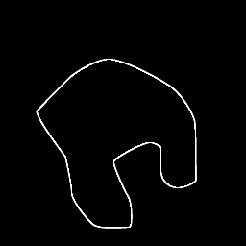
\includegraphics[width=5cm]{images/contour.png}~~~~~~~
  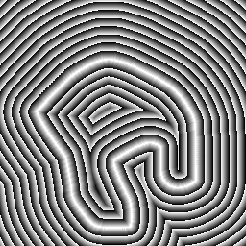
\includegraphics[width=5cm]{images/contour_circ.png} 
\end{center}


\begin{qu}
  Implement a function that digitizes a mathematical shape (see for
  instance the parameteric shapes described in the MicroTutorial
  project) on a digital grid with step $h$. Extract the contour of the
  digital shape (denoted $\partial X$ in the following). 
\end{qu}

\begin{qu}
  Using a distance transformation on the shape and its complement,
  construct an implicit function $f(x,y)$ such that:
  \begin{itemize}
  \item $f(x,y)=0$ if $(x,y)\in \partial X$;
  \item $f(x,y)<0$ (resp. $f(x,y)>0$) if $(x,y)\in X$ (resp. $(x,y)\in
    \bar{X}$) and $f(x,y)$ is the distance between $(x,y)$ and $\partial X$.
  \end{itemize}
\end{qu}
Such function is called a \emph{signed distance transformation} of
$\partial X$.

\begin{qu}
  From this parametrization, implement differential estimators such as
  normal vector field and curvature on boundary points. For example,
  you could consider finite difference analysis of the implicit
  function. As you would see, the estimated quantities could become
  noisy if computations are performed too close to $\partial X$. Propose
  and evaluate a method to smooth the computations (\emph{e.g.} for
  instance using Gaussian convolution with a given parameter $\sigma$
  or using the Voronoi diagram --see \texttt{DGtal::VoronoiMap}-- to
  propagate quantities inside the object).
\end{qu}



\section{Multigrid Analysis}



\begin{qu}
  Perform a complete multigrid convergence evaluation with comparison
  to both expected quantities (available in \textsc{DGtal} for
  implicit shapes, cf  documentation) and estimated ones from other
  estimators (\emph{e.g.} estimators based on maximal DSS
  computations, cf documentation).
\end{qu}

\begin{qu}
  Please discuss about the quality of implicit parametrization based
  estimators (speed, quality...).
\end{qu}

\section{Extensions}


\begin{qu}
  Implement the same estimation on volumetric objects (\emph{i.e.} in
  $\mathbb{Z}^3$). For comparison, please consider normal vector and
  curvature estimators on digital surface implemented in \textsc{DGtal}.  
\end{qu}

\end{document}
